\documentclass[a4paper,12pt]{article} %размер бумаги устанавливаем А4, шрифт 12пунктов
\usepackage[T2A]{fontenc}
\usepackage[utf8]{inputenc}

\usepackage[english,russian]{babel} %используем русский и английский языки с переносами
\usepackage{amssymb,amsfonts,amsmath,mathtext,cite,enumerate,float} %подключаем нужные пакеты расширений

\usepackage[pdftex]{graphicx, color}
\usepackage{subfigure}
\usepackage{color}
\usepackage{listings}

\DeclareGraphicsExtensions{.png,.pdf,.jpg,.mps}
\graphicspath{{pictures/chapter1/}} %путь к рисункам
\usepackage{bmpsize}

\usepackage[nooneline]{caption} \captionsetup[table]{justification=raggedleft} \captionsetup[figure]{justification=centering,labelsep=endash}

\usepackage[left=2cm,right=2cm,top=2cm,bottom=2cm,bindingoffset=0cm]{geometry} % Меняем поля страницы


\begin{document} 
\begin{titlepage}
\newpage

\begin{center}
Государственное образовательное учреждение высшего профессионального образования \\
\vspace{1cm}
\Large<<Московский государственный технический университет имени Н.Э. Баумана>> \\*
(МГТУ им. Н.Э. Баумана) \\*
\hrulefill
\end{center}

\flushright{ФАКУЛЬТЕТ ИНФОРМАТИКИ И СИСТЕМ УПРАВЛЕНИЯ}
\flushright{КАФЕДРА ТЕОРЕТИЧЕСКОЙ ИНФОРМАТИКИ И КОМПЬЮТЕРНЫХ ТЕХНОЛОГИЙ}

\vspace{8em}

\begin{center}
\Large Пояснительная записка \\ к дипломному проекту на тему:
\end{center}

\vspace{2.0em}

\begin{center}
	\Large
\textsc{Множественное выравнивание кодирующих последовательностей ДНК с учетом сдвигов рамки считывания}
\end{center}

\vspace{6em}

\begin{flushleft}
Студент--дипломник \hrulefill Батусов П. В. \\
\vspace{1.5em}
Научный руководитель \hrulefill Страшнов П. В.\\
\vspace{1.5em}
\end{flushleft}

\vspace{\fill}

\begin{center}
Москва 2015
\end{center}

\end{titlepage} 

\renewcommand{\baselinestretch}{1.5}

\renewcommand{\abstractname}{{Аннотация}}
\renewcommand{\abstractname}{\Huge{Аннотация\\[1.5cm]}}
\begin{abstract}

\end{abstract}
\clearpage

\renewcommand{\contentsname}{\centering Содержание}
\tableofcontents % это оглавление, которое генерируется автоматически

% введение
\newpage
\part*{\large \centering ВВЕДЕНИЕ}
\addcontentsline{toc}{part}{ВВЕДЕНИЕ}
\hspace{\parindent} Современная биоинформатика --- это молодая, бурно развивающаяся наука, возникшая в 1976-1978 годах и окончательно оформившаяся в 1980 году со специальным выпуском журнала <<Nucleic Acid Research>> (NAR)~\cite{MironovLect}. По сути, это собрание различных математических моделей и методов в помощь биологам для решения биологических задач, таких как: предсказание пространственной структуры белков, расшифровка структуры ДНК, хранение, поиск и аннотация биологической информации.\\
\indent Основу биоинформатики составляют сравнения. Одна из ключевых задач --- поиск сходства последовательностей. Ее решение позволяет понять функциональное назначение частей геномов, оценить эволюционное расстояние между ними. Кроме этого, различия в генотипах могут объяснить различия в фенотипах.\\
\indent Для того чтобы определить, насколько две последовательности <<похожи>>, используют алгоритмы выравнивания. Они основаны на размещении исходных последовательностей мономеров ДНК, РНК или белков друг под другом таким образом, чтобы было легко увидеть их сходные участки~\cite{WikiPairAlign}. Качество выравнивания оценивают, назначая штрафы за несовпадение букв и за наличие пробелов (когда приходится раздвигать одну последовательность для того, чтобы получить наибольшее число совпадающих позиций), например, через расстояние Левенштейна --- минимальное число элементарных операций (вставка, удаление или замена символа в строке), чтобы превратить одну строку в другую~\cite{Levenshtein}. При сравнении ищется такой вариант выравнивания, чтобы итоговый счет был максимален. В такой постановке задача называется поиском <<глобального выравнивания>>. Необходимо отметить, что для полных геномов глобальное выравнивание не работает, так как при мутации, помимо вставок, удалений и замен, бывают нелинейные перестройки, которые могут менять порядок и ориентацию целых геномных блоков. Для решения, аналогично задаче поиска глобального выравнивания, формулируют задачу поиска <<локального выравнивания>>: для двух произвольных строк $A$ и $B$ найти две самые похожие подстроки и их выравнивание.\\ 
\indent Алгоритмы множественного выравнивания, аналогично алгоритмам парного выравнивания, представляют собой инструмент для установления функциональных, структурных или эволюционных взаимосвязей между биологическими последовательностями.  Несмотря на то, что задача множественного выравнивания была сформулирована более 20 лет назад~\cite{SIAM_Journal}, она до сих пор не теряет своей актуальности. Если говорить о множественном глобальном выравнивании, то, по сравнению с парным выравниванием, практически ничего не меняется: необходимо расставить разрывы в выравниваемых строках таким образом, чтобы <<счет по столбцам>> был максимален. Счет по столбцу можно вести, перебирая все пары символов. Множественное локальное выравнивание обобщить на многомерный случай не так просто. Во-первых, какие-то подстроки могут быть не во всех последовательностях. Во-вторых, последовательности могут содержать дуплицированные участки. Поэтому для решения такой задачи необходимо более точно сформулировать условия выравнивания.\\ 
\indent Таким образом, две главные составляющие автоматических методов выравнивания --- это непосредственно алгоритм и функция оценки качества полученного результата. На сегодняшний день можно выделить два основных алгоритма выравнивания биологических последовательностей: алгоритм Нидлмана-Вунша и алгоритм Смита-Ватермана. Они представляют собой классический пример задачи динамического программирования. Существуют различные их модификации, использующие эвристики для уменьшения количества шагов алгоритма или требуемого объема памяти, однако,эти методы строят выравнивание без сохранения открытых рамок считывания. В погоне за лучшим счетом происходит потеря биологического смысла результата.\\ 
\indent Задача множественного выравнивания с учетом открытых рамок считывания требует других, более сложных подходов. Один из существующих методов решения: построить выравнивание исходной нуклеотидной последовательности на аминокислотном уровне~\cite{MACSE}. У такого подхода есть несколько проблем. Во-первых, появление преждевременного стоп-кодона. Во-вторых, так как каждая последовательность переводится с одной и той же рамкой считывания от начала и до конца, то присутствие единственного дополнительного нуклеотида приведет к аномальному переводу и выравниванию.

% глава 1
\newpage

\section[Обзор предметной области]{\large \centering Обзор предметной области}
\hspace{\parindent} Выравнивание аминокислотных или нуклеотидных последовательностей --- это процесс сопоставления сравниваемых последовательностей для такого их взаиморасположения, при котором наблюдается максимальное количество совпадений аминокислотных остатков или нуклеотидов~\cite{AlignmentClustal}. Различают два вида выравнивания: парное (выравнивание двух последовательностей ДНК, РНК или белков) и множественное (выравнивание трех и более последовательностей). 

\subsection[Существующие методы поиска гомологий в биологических последовательностях]{\large Существующие методы поиска гомологий в биологических последовательностях}
\hspace{\parindent} В генетике под гомологиями понимаются участки белков или ДНК, имеющие сходную последовательность аминокислот или нуклеотидов. Обычно существа, у которых есть гомологичные участки белков или ДНК, имеют общего предка, от которого они и получили такой участок. Поскольку в процессе эволюции ДНК подвергается мутациям, эти участки не обязательно идентичны. В них могут быть случайно заменены, добавлены или удалены нуклеотиды или аминокислоты. Некоторые мутации, такие, как транслокации и инверсии, приводят к изменениям, затрагивающим большие участки генома. Такие мутации сложно учитывать, поскольку локальное сходство проверять легче, чем глобальное, а в результате глобальных мутаций участки ДНК могут быть соединены в непредсказуемом порядке. %Поэтому существующие методы поиска гомологий умеют находить участки (подстроки) двух последовательностей, которые отличаются не очень сильно.

\subsubsection[Алгоритм Нидлмана-Вунша]{\large Алгоритм Нидлмана-Вунша}
\hspace{\parindent} Одним из наиболее распространенных алгоритмов выравнивания является алгоритм Нидлмана-Вунша~\cite{NWalgo}, основанный на двумерном динамическом программировании. Для своей работы алгоритм использует матрицу сходства, которая указывает, насколько схожими можно считать разные нуклеотиды. Использование матрицы позволяет придавать разный вес разным заменам нуклеотидов. Например, поскольку транзиции более вероятны, чем трансверсии, логично считать последовательности, отличающиеся заменой пурина на пурин или пиримидина на пиримидин, более схожими, чем те, которые отличаются заменой пурина на пиримидин или наоборот. Обычно используется симметричная матрица, однако, применение несимметричной матрицы позволяет различать замены в одну и в другую стороны. На рисунке~\ref{ris:ReplaceMatrix} представлен пример матрицы сходства. Здесь А, Г, Т и Ц обозначают, соответственно, аденин, гуанин, тимин и цитозин, а числа в матрице указывают степень сходства между двумя нуклеотидами.

\begin{figure}[h]
	\center{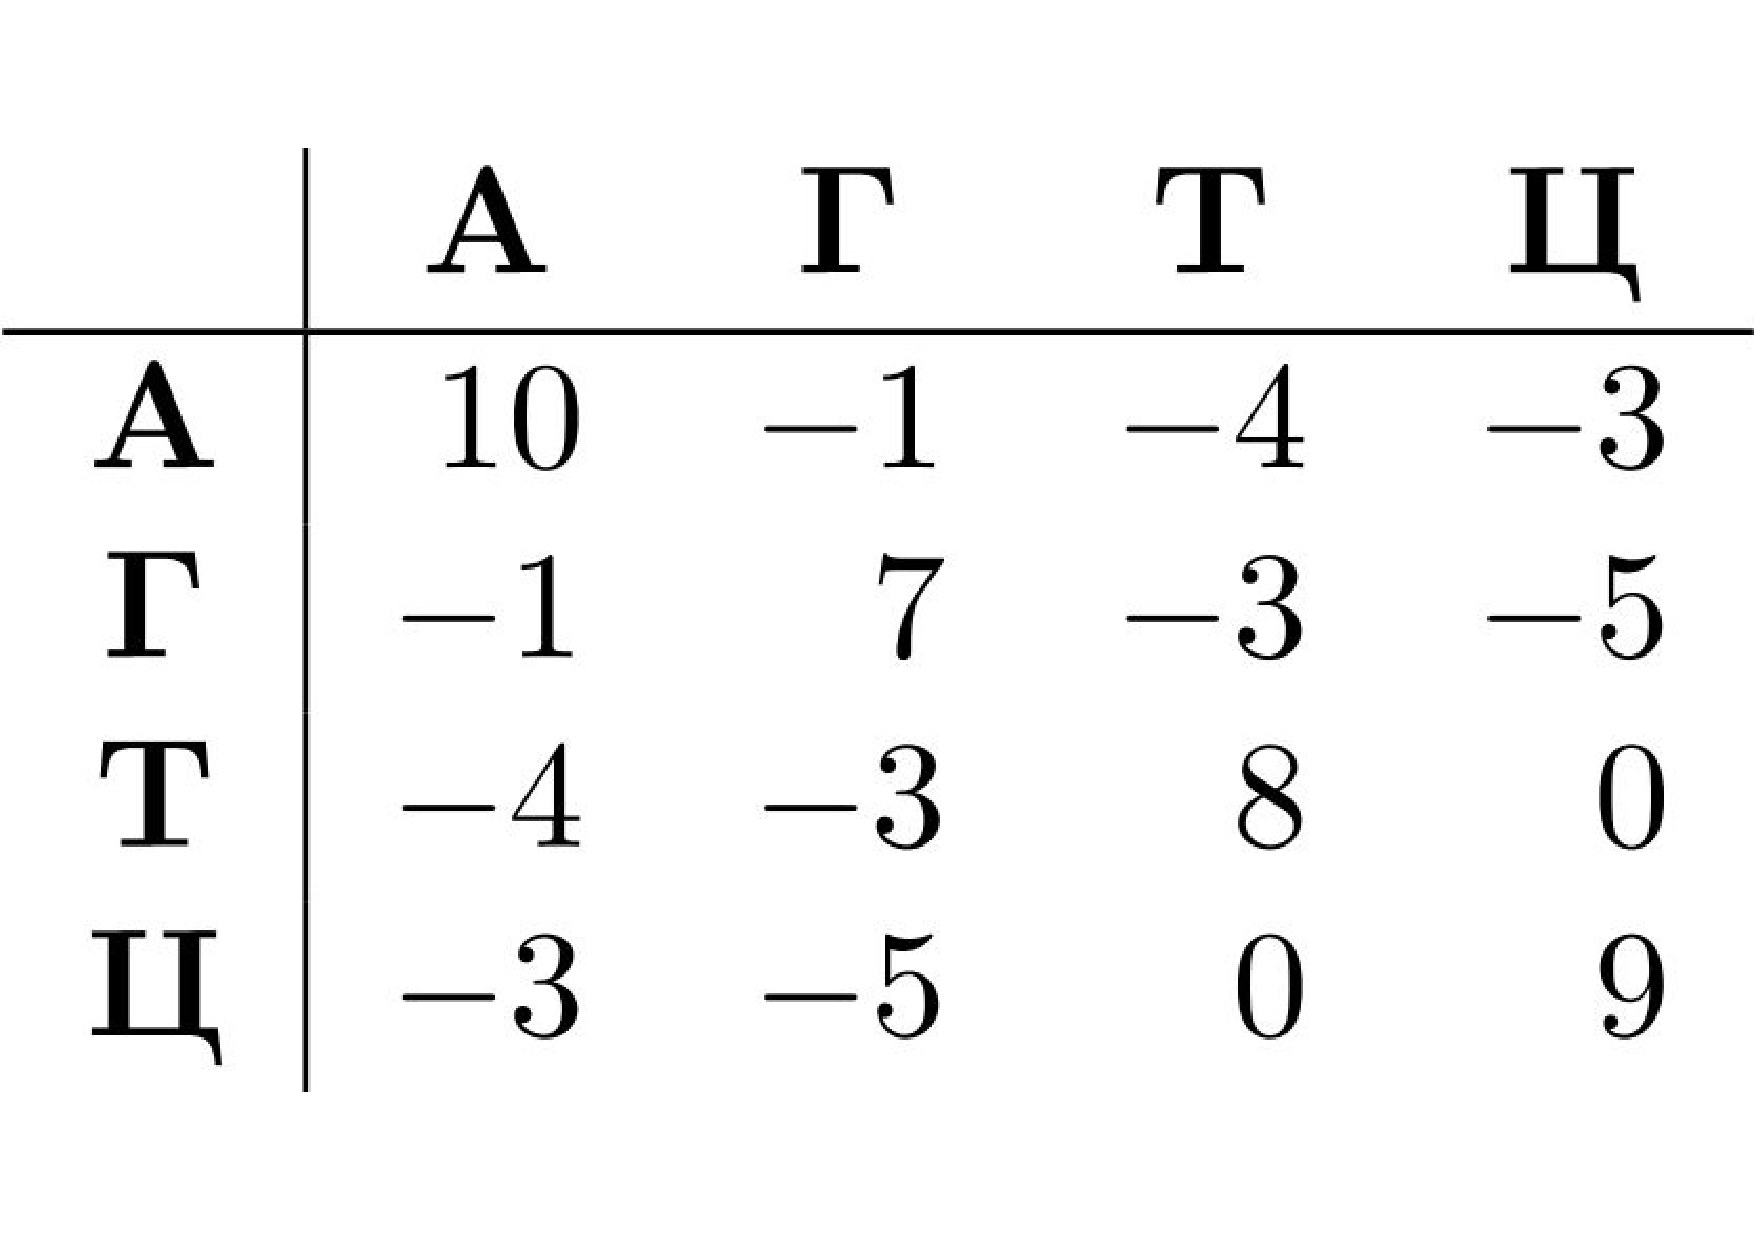
\includegraphics[width=0.4\linewidth]{RM.pdf}}
	\caption{Пример матрицы сходства}
	\label{ris:ReplaceMatrix}
\end{figure}

\indent Еще один параметр алгоритма --- штраф за разрыв последовательности. Он может выражаться произвольной функцией от длины и/или направления разрыва. Для определенности будем рассматривать линейный штраф за разрыв, определяющийся параметром $d$ (за разрыв длинны $n$ будет начислен штраф $d \cdot n$).\\
\indent На вход алгоритм получает матрицу сходства $S$, параметр штрафа $d$ и две последовательности (строки), которые необходимо выровнять. Для получения результата выполняется построение матрицы $F_{i,j}$ , где $i$ и $j$ изменяются от нуля до длины, соответственно, первой и второй строк. Вначале алгоритм инициализирует $F_{i,0}$ и $F_{0,j}$ равными, соответственно, $d \cdot i$ и $d \cdot j$ для всех $i$ и $j$. Затем происходит вычисление оставшихся элементов матрицы по формуле~\ref{eq:N_W}.

\begin{equation}\label{eq:N_W}
F_{i,j} = max\left\{
	\begin{aligned}
		& F_{i-1,j-1} + S_{A_i,B_j}\\
		& F_{i-1,j} + d\\
		& F_{i,j-1} + d
	\end{aligned}
	\right.
\end{equation}

\indent  После того, как матрица посчитана, необходимо определить, каким путем появилось значение в правом нижнем углу. Например, если $F_{i,j} = F_{i-1,j-1} +S_{A_{i-1},B_{j-1}}$, то элемент $(i, j)$ появился из элемента $(i - 1, j - 1)$, и т. д. Элементы в верхней строке произошли из элементов левее себя, элементы из левого столбца --- из элементов выше себя. Переход вида $(i, j) \rightarrow (i - 1, j - 1)$ означает, что $i$-му символу в первой строке соответствует $j$-й символ во второй строке. Переход вида $(i, j) \rightarrow (i - 1, j)$ означает, что $i$-му символу первой строки ничего не соответствует, а переход $(i, j) \rightarrow (i, j - 1)$ --- что $j$-му символу второй строки ничего не соответствует. Путь в матрице от левого верхнего угла к правому нижнему даст искомое выравнивание последовательностей.\\
\indent Очевидно, что алгоритм всегда ищет выравнивание с максимальным счетом, так как строя матрицу $F$, он рассматривает всевозможные варианты размещения одной строки относительно другой. Время работы и количество используемой памяти пропорционально произведению длин последовательностей.

\subsubsection[Алгоритм Смита-Ватермана]{\large Алгоритм Смита-Ватермана}
\hspace{\parindent} Алгоритм Смита-Ватермана~\cite{SWalgo} аналогичен алгоритму Нидлмана-Вунша, но решает задачу локального выравнивания: находит подстроки первой и второй строк, обладающие максимальным сходством.\\
\indent На вход алгоритм получает матрицу сходства $S$, две последовательности и два вектора $I$ и $D$, вектор стоимостей добавления и вектор стоимостей удаления, соответственно. Элементы матрицы $F_{i,0}$ и $F_{0,j}$ инициализируются нулями.  Вычисление оставшихся элементов происходит по формуле~\ref{eq:S_W}.

\begin{equation}\label{eq:S_W}
F_{i,j} = max\left\{
	\begin{aligned}
		& F_{i-1,j-1} + S_{A_i,B_j}\\
		& F_{i-1,j} + D_{A_i}\\
		& F_{i,j-1} + I_{B_j}\\
		& 0
	\end{aligned}
	\right.
\end{equation}

\indent Для получения выравнивания необходимо найти максимальный элемент в матрице. Если переходить от этого элемента по цепочке предыдущих, то путь закончится в каком-то нулевом элементе. Индексы этих двух элементов равны индексам начал и концов подстрок: первые индексы --- в первой строке, вторые --- во второй. Путь интерпретируется так же, как и в алгоритме Нидлмана-Вунша.\\
\indent Видно, что оба алгоритма похожи друг на друга. Они имеют одинаковую сложность и затраты по памяти, что делает такие алгоритмы неприемлемыми для работы с большим количеством генетического материала.

\subsubsection[Алгоритм Хиршберга]{\large Алгоритм Хиршберга}
\hspace{\parindent} Оба предыдущих алгоритма требуют объем памяти, пропорциональный произведению длин выравниваемых последовательностей, что затрудняет обработку больших строк, поэтому очень важно иметь методы, уменьшающие затраты памяти без критического увеличения времени счета. В 1975 году был предложен алгоритм Хиршберга, значительно сокращающий затраты памяти~\cite{Hirshberg}. Он позволяет вычислять оптимальное выравнивание строк длины $n$ и $m$, используя $O(n+m)$ количество памяти, но примерно вдвое большее времени счета по сравнению с алгоритмом Нидлмана-Вунша.\\
\indent Идея алгоритма состоит в том, что одна из двух входных последовательностей разбивается на две части, и исходная задача сводится к двум, меньшим, задачам выравнивания второй входной последовательности с каждой из частей. Решение подзадач осуществляется путем аналогичного сведения к подзадачам. На рисунке~\ref{ris:Hirshberg} показана схема разбивки задачи на две подзадачи: верхнюю, которая решается в прямоугольнике $A$ исходной таблицы, и нижнюю --- в прямоугольнике $B$. Последовательности имеют длины $n$ и $m$, соответственно. Для разбиения каждой задачи на подзадачи необходимо вычислить значение $k^*$. При этом используется объем памяти, линейно зависящий от $m$. Верхняя задача заключается в выравнивании строки с длинами не больше $n/2$ и $k^*$, а нижняя – с длинами не больше $n/2$ и $m-k^*$. 

\begin{figure}[h]
	\center{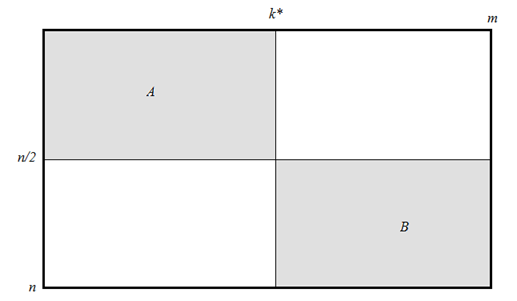
\includegraphics[width=0.7\linewidth]{hirshberg.png}}
	\caption{Разделение задачи выравнивания на две подзадачи}
	\label{ris:Hirshberg}
\end{figure}

\indent Для представления задач в алгоритме Хиршберга можно использовать бинарные деревья~\cite{HirshbergParallel}. Узлам дерева соответствуют подзадачи, которые заключаются в выравнивании меньших подпоследовательностей. Каждый узел дерева хранит в памяти границу прямоугольной области, в которой решается соответствующая задача динамического программирования. Дерево в процессе работы алгоритма строится по уровням. Сначала оно состоит только из корневого узла, который соответствует прямоугольнику $[0,0]\times[n,m]$. Создание двух узлов эквивалентно разбиению задачи на две подзадачи и разделению области решения на две, меньшего размера.\\
\indent Алгоритм Хиршберга заключается в обходе полного дерева всех подзадач. Результат выравнивания можно будет получить, если пройтись по листьям построенного дерева (рисунок~\ref{ris:HirshbergExample}). Для оптимизации вычислений можно выполнять обход (решение подзадач) только части вершин дерева: тех, которые удалены от корня на величину, не превосходящую заранее заданную константу $h$ --- максимальную глубину обхода дерева. При достижении глубины дерева $h$ или минимального размера прямоугольника применяется алгоритм Нидлмана-Вунша, который работает вдвое быстрее алгоритма Хиршберга.

\begin{figure}[h]
	\center{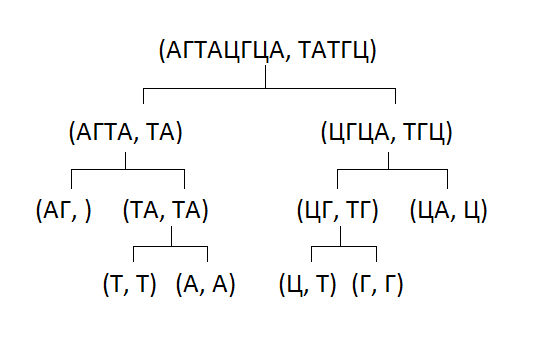
\includegraphics[width=0.7\linewidth]{hirshberg-example.png}}
	\caption{Дерево подзадач для алгоритма Хиршберга}
	\label{ris:HirshbergExample}
\end{figure}

\indent Дополнительное ускорение можно получить за счет распараллеливания. Заметим, что на каждом шаге алгоритма полученные подзадачи никак не связаны между собой, и, следовательно, их решения могут вычисляться в отдельных потоках.

\subsection[Представление генетической информации в электронном виде]{\large Представление генетической информации в электронном виде}
\hspace{\parindent} Поскольку различных нуклеотидов и стандартных аминокислот немного, для их кодирования используют один символ --- первую букву из названия. С другой стороны, названия многих аминокислот начинаются с одинаковых букв, поэтому для кодирования приходится использовать те, которые остаются незанятыми.

\subsubsection[Формат FASTA]{\large Формат FASTA}
\hspace{\parindent} В формате FASTA~\cite{FASTAformat} строчка, начинающаяся с символа '>', называется строкой описания. Она содержит имя последовательности и некоторую дополнительную информацию, предназначенную для идентификации. Другие строки, начинающиеся с символа ';', являются комментариями и игнорируются. За строкой описания следует код последовательности. При кодировании нуклеотидов буквами A, C, G, T и U кодируют, соответственно, аденин, цитозин, гуанин, тимин и урацил. Обычно, длинные последовательности разбивают на несколько строк длиной не более 80 символов --- это не правило формата, но представление данных таким образом выглядит более наглядно для человека.

\subsubsection[Формат FASTQ]{\large Формат FASTQ}
\hspace{\parindent} FASTQ --- формат представления биологической последовательности совместно с данными о качестве. Он используется для представления данных секвенирования. При кодировании уровней качества используются символы из таблицы ASCII от '!' до '\textasciitilde'.\\
\indent Существует два различных способа выражать уровень качества через вероятность ошибки: формулы~\ref{eq:FASTQ:quality1} и~\ref{eq:FASTQ:quality2}, где $Q$ --- уровень качества, а $p$ --- вероятность, что элемент последовательности ошибочный. При малых значениях $p$ эти способы дают практически идентичные результаты, но с ростом $p$ уровни качества начинают заметно различаются (рисунок~\ref{ris:FASTQscore}).

\begin{equation} \label{eq:FASTQ:quality1}
Q = -10 \cdot \log_{10} p
\end{equation}
\begin{equation} \label{eq:FASTQ:quality2}
Q = -10 \cdot \log_{10} \dfrac{p}{(1-p)}
\end{equation}
\begin{figure}[h]
	\center{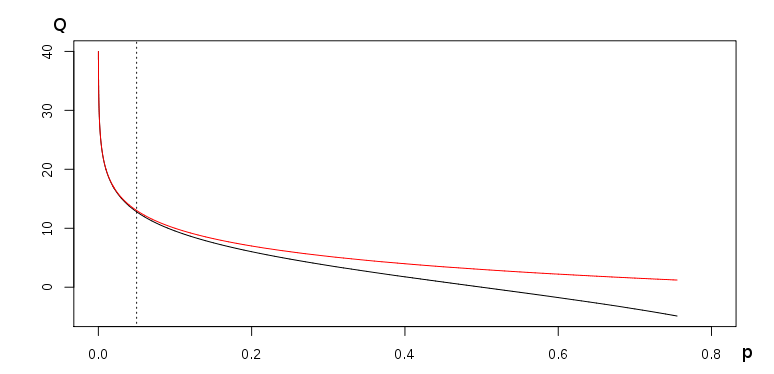
\includegraphics[width=0.9\linewidth]{FASTQscore.png}}
	\caption{График уровней качества для формул~\ref{eq:FASTQ:quality1} (красная) и~\ref{eq:FASTQ:quality2} (черная)}
	\label{ris:FASTQscore}
\end{figure}

\indent Файл в формате FASTQ содержит четыре строки для каждой последовательности. Первая строка начинается с символа '@', после которого идет описание последовательности (строка описания). Следующая строка содержит набор символов, кодирующих саму последовательность аналогично формату FASTA. За ней идёт строка, начинающаяся с символа '+', содержащая дополнительное описание последовательности. Последняя строка содержит уровни качества. 

\subsubsection[Формат GenBank]{\large Формат GenBank}
\hspace{\parindent} Запись в формате GenBank состоит из двух секций: секции аннотации и секции данных~\cite{GenBankFormat}. В первой хранится всевозможная информация о последовательности: из какого организма получена, ссылки на другие работы, различные примечания, а во второй --- сама последовательность, аналогично формату FASTA. Начало секции аннотации отмечается кодовым словом <<LOCUS>>, а секция данных начинается со слова <<ORIGIN>>. В конце описания последовательности ставится специальный маркер <<//>>. Формат GenBank, по сравнению с форматами FAST и FASTQ, позволяет представить больше дополнительной информации о последовательности.

% заключение
\newpage
\part*{\large \centering ВЫВОДЫ}
\addcontentsline{toc}{part}{ВЫВОДЫ}
\hspace{\parindent} Целью настоящей работы являлось создание приложения для построения множественных выравниваний кодирующих последовательностей ДНК с учетом сдвигов рамки считывания. Поставленная задача была успешно выполнена, кроме этого, разработанная программа в результате тестирования показала хороший прирост скорости по сравнению с существующим аналогом. Также были созданы статические библиотеки парного и множественного выравниваний для использования в сторонних проектах. Приложение написано на языке программирования C++ и является кроссплатформенным. Для упрощения работы дополнительно к программе был создан веб-интерфейс.\\
\indent Дальнейшее развитие проекта предполагает поиск новых подходов для улучшения качества получаемого ответа. При объединении профилей, разработанный алгоритм не пересматривает предыдущие решения. Любой поставленный разрыв будет присутствовать в итоговом выравнивании. Возможно, дополнительный набор проверок и перевыравниваний сделает ответ более целым и, соответственно, более качественным.

% оглавление
\clearpage
\newpage
\bibliographystyle{utf8gost705u}  %% стилевой файл для оформления по ГОСТу
\begin{flushleft}
\bibliography{biblio}     %% имя библиографической базы (bib-файла) 
\end{flushleft}

\end{document}